
\section{Malware Hash Detection in Zeek}
\subsection{How It Works}
The Zeek script integrates with Team Cymru's Malware Hash Registry to enhance network security monitoring by identifying files with hash values known to be associated with malware. The process is outlined as follows:

\begin{itemize}

    \item \textbf{Initialization :} The script initializes by loading essential frameworks for file handling and notice management, setting the groundwork for its operations.
    \item \textbf{Notice Extension :} It extends Zeek's notice mechanism to include a new type specifically for malware hash matches, facilitating targeted alerts.
    \item \textbf{File Filtering :} File downloads are filtered by MIME type, focusing the analysis on file formats commonly associated with malware dissemination.
    \item \textbf{Malware Hash Lookup :} For each relevant file, the script performs a DNS TXT lookup against the Malware Hash Registry using the file's SHA-1 hash as the query, efficiently leveraging external threat intelligence.
    \item \textbf{Lookup Evaluation :} The lookup response, containing the detection rate and first detection date, is evaluated against a predefined threshold to determine the file's potential threat level.
    \item \textbf{Notice Generation :} If the detection criteria are met, a notice is generated, including the malware detection rate, the URL for further information, and the file's last seen date, thereby informing the network administrator of potential security threats.
    \item \textbf{Network Defense Enhancement :} This integration allows for an automated, real-time response to the transmission of potentially malicious files, enhancing the network's defensive posture against malware.
\end{itemize}


\subsection{Detect-MHR Script:}
\begin{lstlisting}[language=Python, caption=detect-MHR.zeek]
##! Detect file downloads that have hash values matching files in Team
##! Cymru's Malware Hash Registry (https://www.team-cymru.com/mhr.html).

@load base/frameworks/files
@load base/frameworks/notice
@load frameworks/files/hash-all-files

module TeamCymruMalwareHashRegistry;

export {
	redef enum Notice::Type += {
		Match
	};

	## File types to attempt matching against the Malware Hash Registry.
	option match_file_types = /application\/x-dosexec/ |
	                         /application\/vnd\.ms-cab-compressed/ |
	                         /application\/pdf/ |
	                         /application\/x-shockwave-flash/ |
	                         /application\/x-java-applet/ |
	                         /application\/jar/ |
	                         /video\/mp4/;


	option match_sub_url = "https://www.virustotal.com/gui/search/%s";
	option notice_threshold = 10;
}


function do_mhr_lookup(hash: string, fi: Notice::FileInfo)
	{
	local hash_domain = fmt("%s.malware.hash.cymru.com", hash);
	when [hash, fi, hash_domain] ( local MHR_result = lookup_hostname_txt(hash_domain) )
		{
		local MHR_answer = split_string1(MHR_result, / /);

		if ( |MHR_answer| == 2 )
			{
			local mhr_detect_rate = to_count(MHR_answer[1]);
			if ( mhr_detect_rate >= notice_threshold )
				{
				local mhr_first_detected = double_to_time(to_double(MHR_answer[0]));

				local readable_first_detected = strftime("%Y-%m-%d %H:%M:%S", mhr_first_detected);

				local message = fmt("Malware Hash Registry Detection rate: %d%%  Last seen: %s", mhr_detect_rate, readable_first_detected);

				local virustotal_url = fmt(match_sub_url, hash);

				local n: Notice::Info = Notice::Info($note=Match, $msg=message, $sub=virustotal_url);
				Notice::populate_file_info2(fi, n);
				NOTICE(n);
				}
			}
		}
	}

event file_hash(f: fa_file, kind: string, hash: string)
	{
	if ( kind == "sha1" && f?$info && f$info?$mime_type &&
	     match_file_types in f$info$mime_type )
		do_mhr_lookup(hash, Notice::create_file_info(f));
	}

 \end{lstlisting}

 \subsection{Detect-MHR Script Explanation :}
 \begin{enumerate}
    \item \textbf{Module and Dependencies} (Lines 4-8) : The script introduces the `TeamCymruMalwareHashRegistry` module and includes necessary Zeek frameworks for file operations and notice generation.
    \item \textbf{Notice Type Extension} (Lines 11-12) : Extends `Notice::Type` with `Match` to signify malware hash matches.
    \item \textbf{File Type Filtering} (Lines 16-22) : Defines `match\_file\_types` to specify MIME types of interest, including executables, archives, PDFs, Flash, Java applets, and MP4 videos.
    \item \textbf{Malware Information URL} (Line 25) : The `match\_sub\_url` option formats a URL to VirusTotal, substituting `%s` with the file's SHA-1 hash for further investigation.
    \item \textbf{Detection Threshold} (Line 26) : Sets a `notice\_threshold` to determine the minimum detection rate by antivirus engines for generating a notice.
    \item \textbf{Malware Hash Lookup} (Lines 30-48) : Implements `do\_mhr\_lookup` to query the hash in Team Cymru's Malware Hash Registry via DNS TXT lookup.
    \item \textbf{Handling Lookup Results} (Lines 50-52) : Processes lookup results, generating a notice if the detection rate exceeds the set threshold, including the rate, last seen date, and a VirusTotal link.
    \item \textbf{File Hash Event} (Lines 58-62) : The `file\_hash` event initiates the malware hash lookup for SHA-1 hashes of files matching the specified MIME types.
\end{enumerate}

\subsection{Simulation : }
Here is the link to VirusTotal: \href{https://www.virustotal.com/gui/search/a38b59afb1f03b2c2cfc14ae5a953d8e5fd6b56d}{VirusTotal}\\
Here is the link to PCAP file:
\href{https://www.malware-traffic-analysis.net/tutorials/index.html}{malware-traffic-analysis}\\\\
\begin{itemize}
    \item To begin the analysis, the malicious pcap file is processed using the detect-MHR.zeek script, specifically designed for malware hash detection.
\end{itemize}

\begin{figure}[h!]
    \centering
    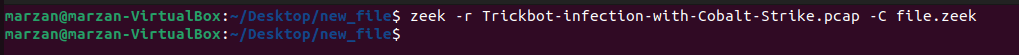
\includegraphics[width=1\linewidth]{images//file_malware/file_malware_1.png}
    \caption{Running PCAP with Script}
    \label{fig:enter-label}
\end{figure}

\begin{itemize}
    \item The notice.log entries highlight malware detections with the following critical information: the detection rate, the last seen date, and a link to VirusTotal for further investigation. For instance, one entry shows a 3\% detection rate for malware last seen on 2021-06-22, with a corresponding VirusTotal search link for the hash bdfb8b29614001dfe9922524c910ee4badb0e6fc. Another entry indicates a 32\% detection rate for malware last seen on 2021-06-04, linked to the hash 9b4025714911d509a67423ed8beffbc49e54845d on VirusTotal. These details facilitate a deeper analysis of the detected threats.
\end{itemize}
\begin{figure}[H]
    \centering
    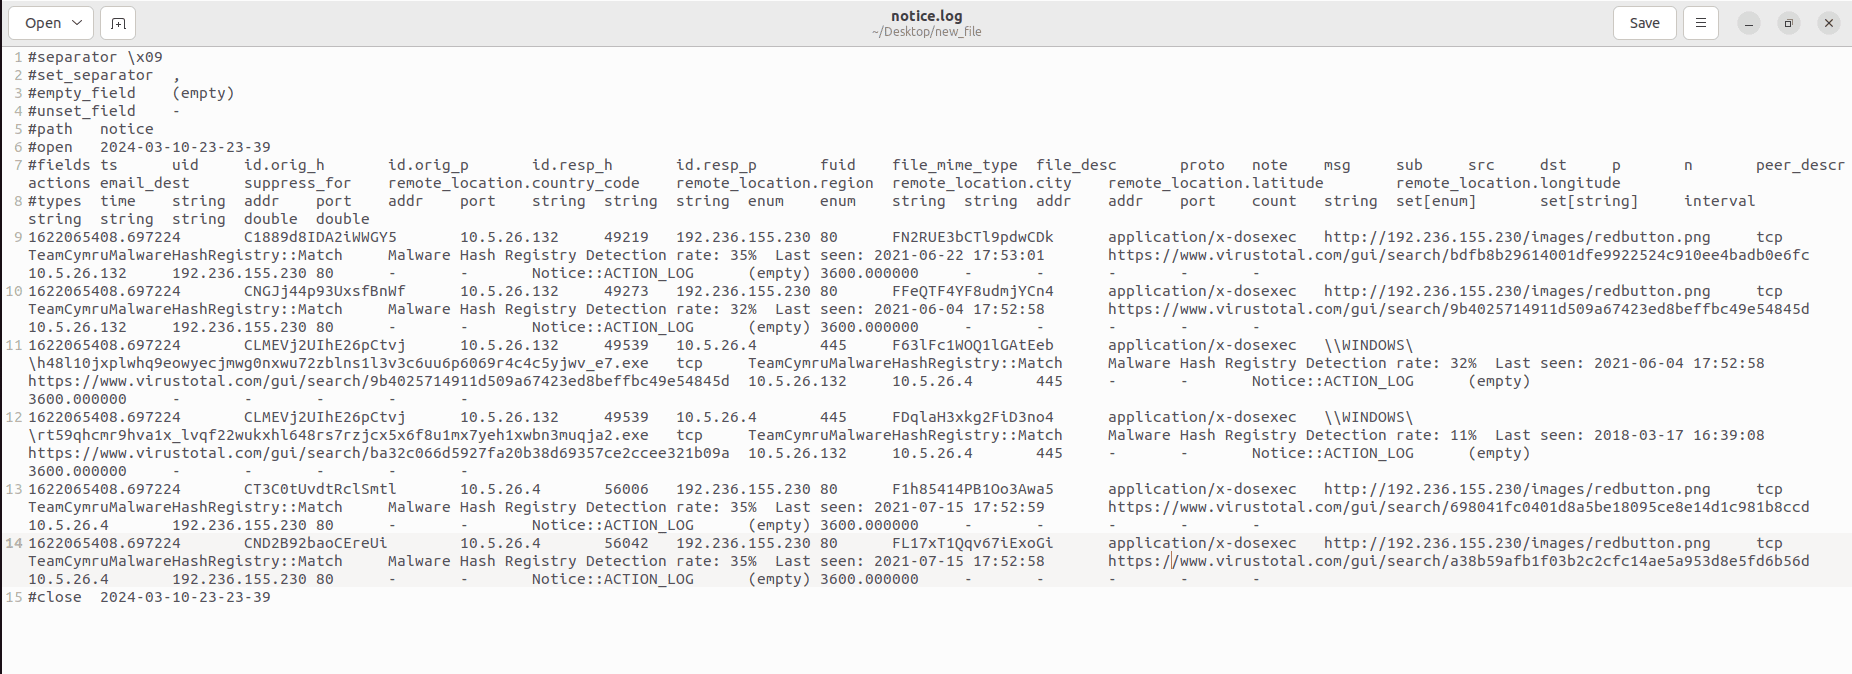
\includegraphics[width=1\linewidth]{images//file_malware/file_malware_2.png}
    \caption{notice.log}
    \label{fig:enter-label}
\end{figure}

\begin{itemize}
    \item These detection logs can be viewed in a tabular format within the BRIM application, providing a user-friendly interface for detailed analysis.
\end{itemize}
\begin{figure}[H]
    \centering
    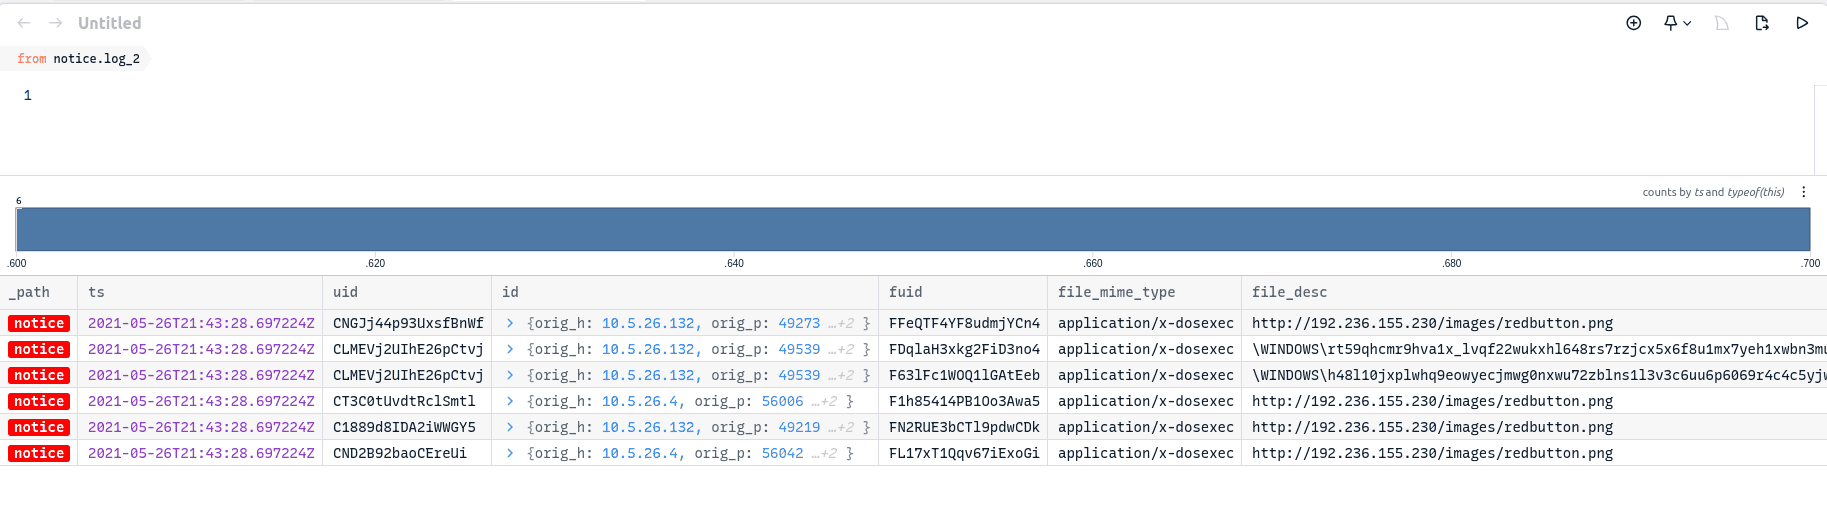
\includegraphics[width=1\linewidth]{images//UDP_reflection/file_malware_6.png}
    \caption{notice.log in BRIM}
    \label{fig:enter-label}
\end{figure}

\begin{figure}[H]
    \centering
    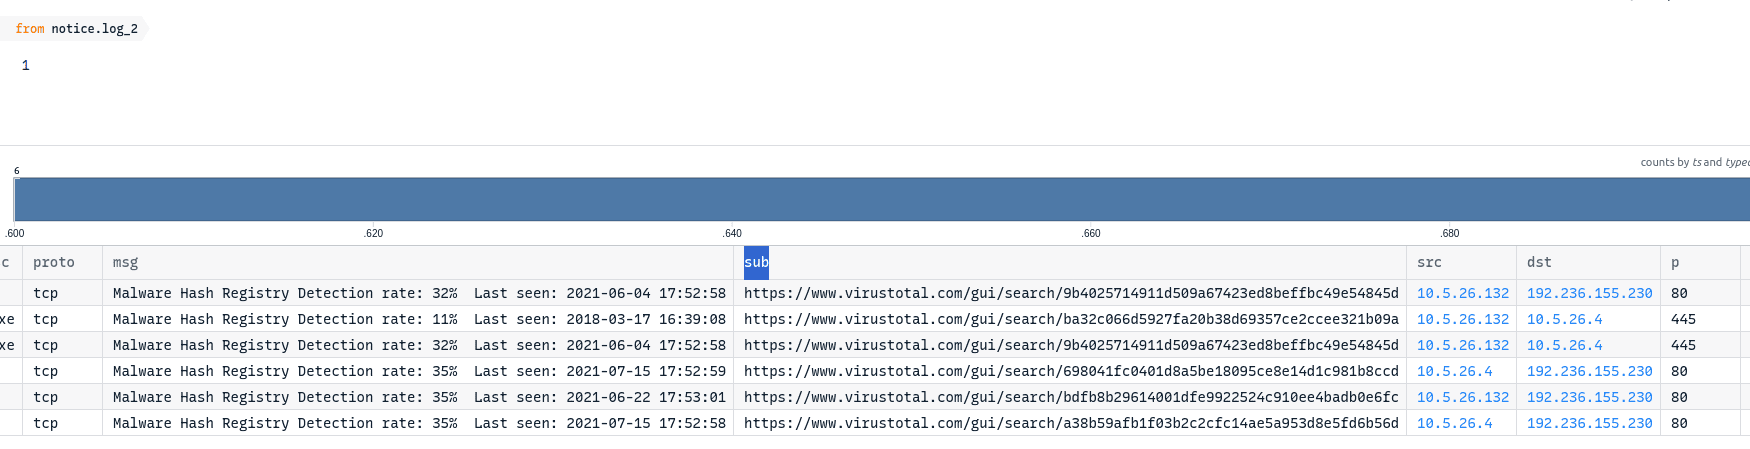
\includegraphics[width=1\linewidth]{images//UDP_reflection/file_malware_7.png}
    \caption{notice.log in BRIM}
    \label{fig:enter-label}
\end{figure}

\begin{itemize}
    \item Within BRIM, each entry's detailed information is accessible, including path, timestamp, unique identifiers, file information, MIME type, descriptions, protocols, notices, messages, source and destination details, and more. This detailed view aids in a comprehensive analysis of each detected event.
\end{itemize}
\begin{figure}[H]
    \centering
    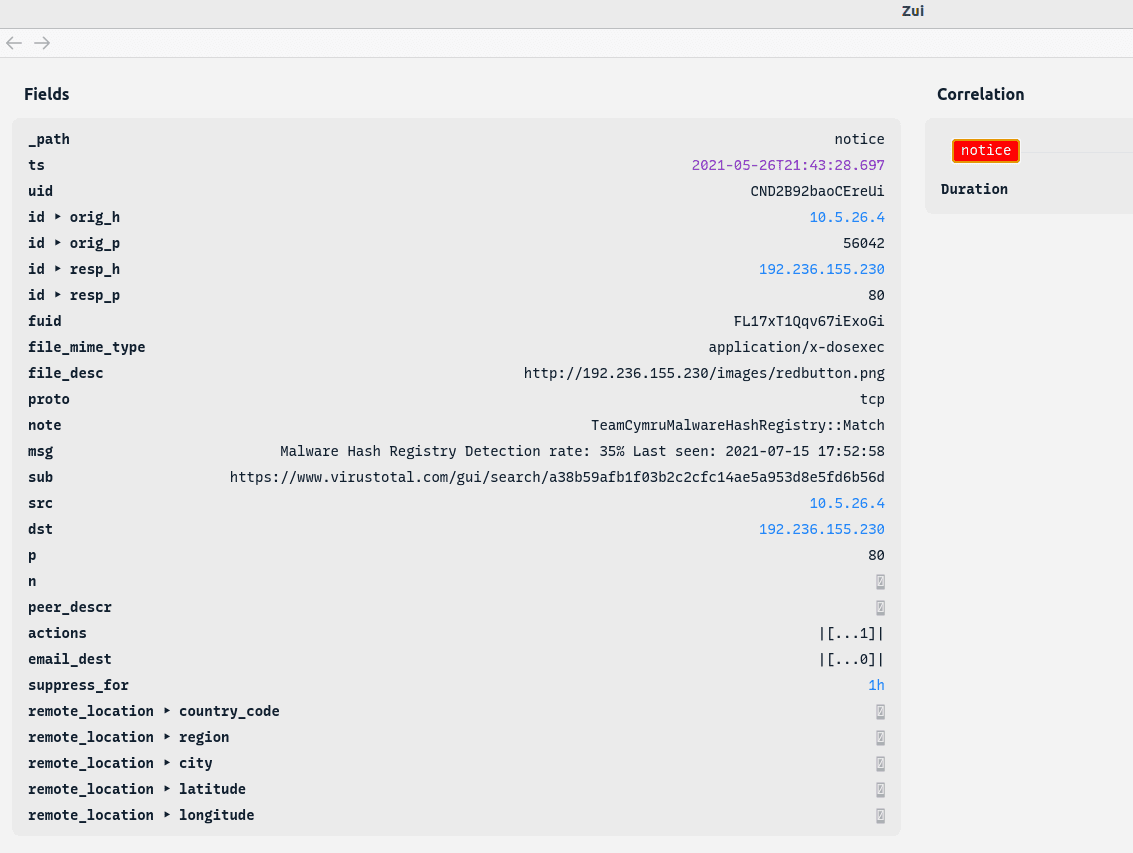
\includegraphics[width=0.7\linewidth]{images//file_malware/file_malware_3.png}
    \caption{Entries of notice.log in BRIM}
    \label{fig:enter-label}
\end{figure}

\begin{itemize}
    \item Following the links in the notice.log to VirusTotal provides a detailed security report for each file hash, including the community score, detection rates by various security vendors, and additional malware characteristics. This external validation offers insights into the potential threats and the behavior of the detected files.
\end{itemize}
\begin{figure}[H]
    \centering
    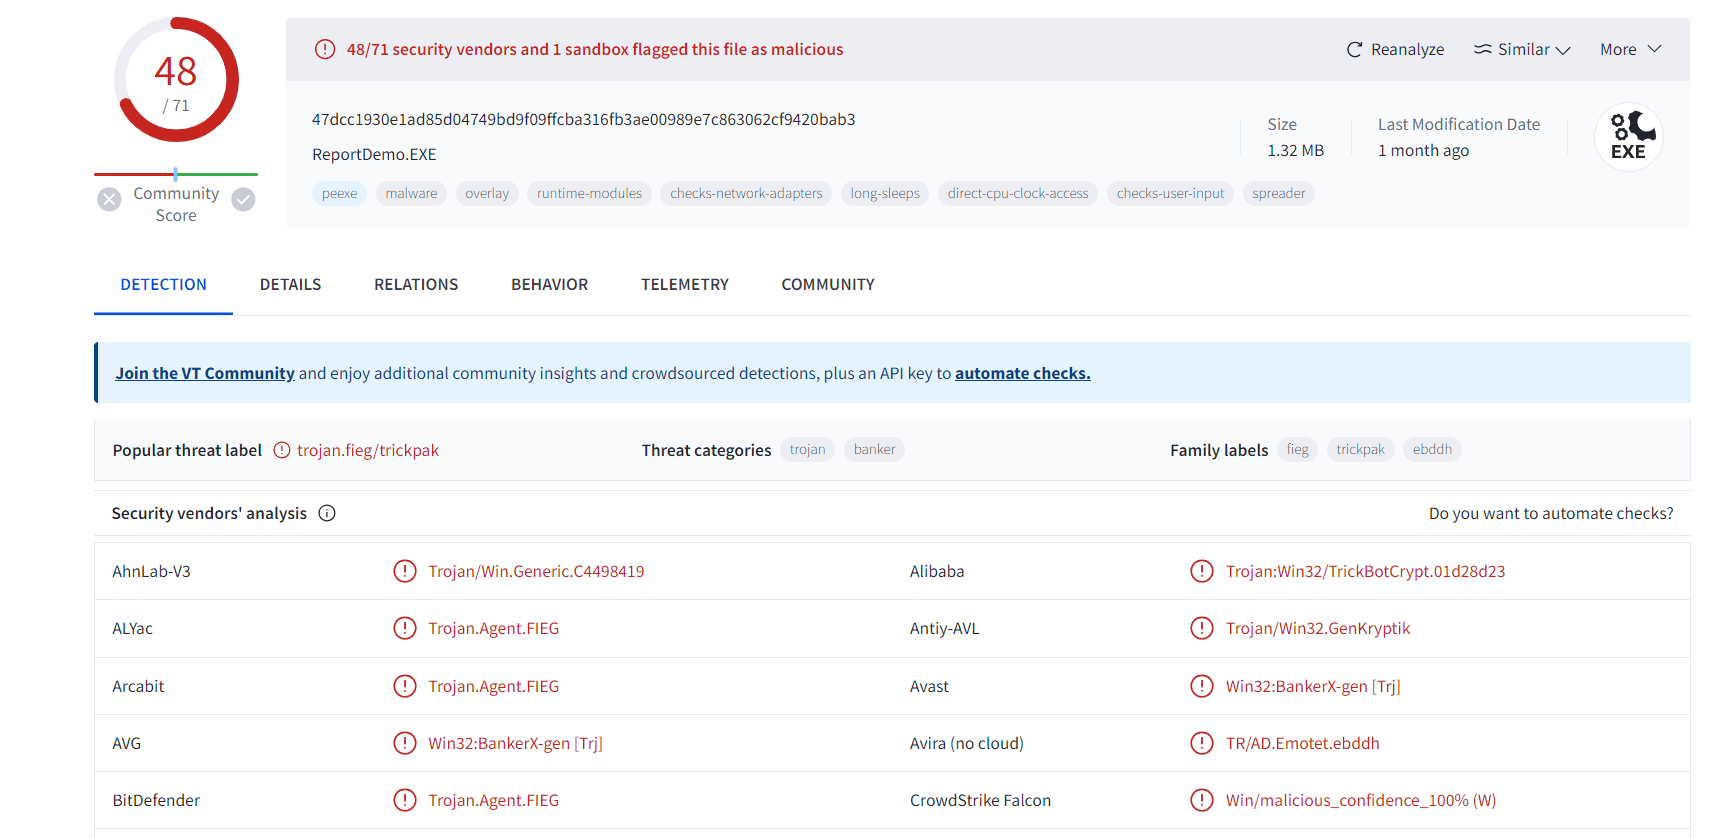
\includegraphics[width=1\linewidth]{images//file_malware/file_malware_4.png}
    \caption{VirusTotal Page Showing Malicious Percentage}
    \label{fig:enter-label}
\end{figure}

\begin{itemize}
    \item The VirusTotal reports also reveal basic file properties such as MD5, SHA-1, and SHA-256 hashes, providing an authoritative fingerprint of the files for cross-reference and further investigation into their origins, distribution, and impact.
\end{itemize}
\begin{figure}[H]
    \centering
    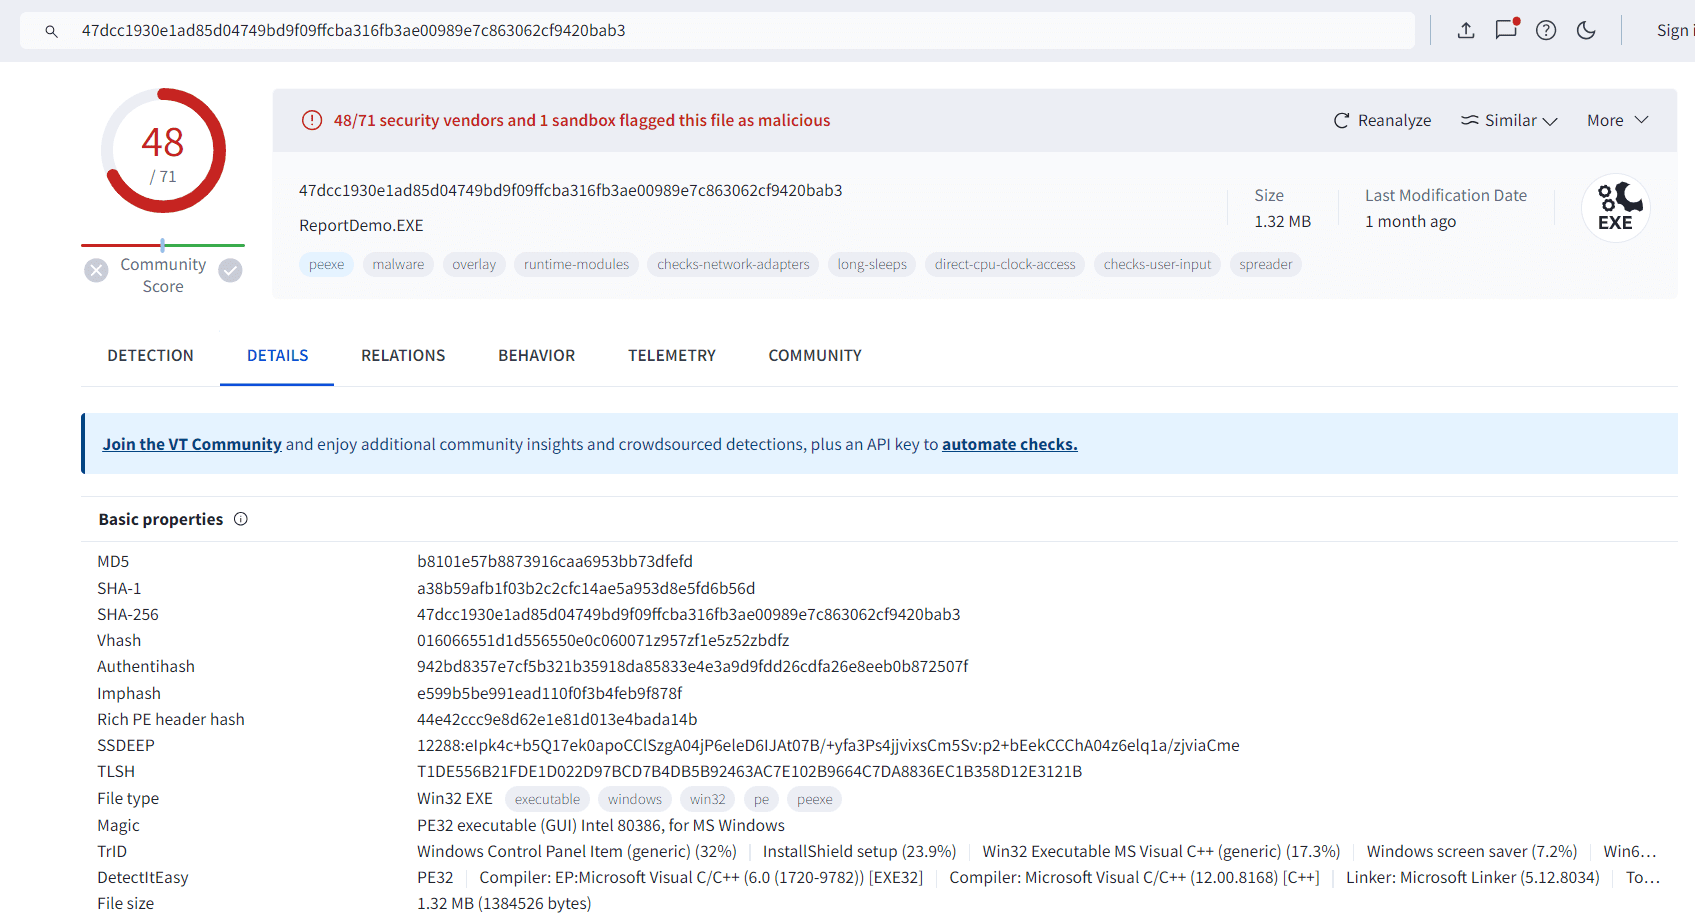
\includegraphics[width=1\linewidth]{images//file_malware/file_malware_5.png}
    \caption{VirusTotal Page Showing File Info}
    \label{fig:enter-label}
\end{figure}
